\section{The ULTRACAM instrument} 

The Ultracam high speed photometry camera (hereafter, ULTRACAM) had its `first-light' at the William Herschel Telescope (WHT) on the 16 May 2002. Since then it has been used on many occasions at three telescopes, namely the William Herschel Telescope (WHT), La Palma, Islas Canarias, the Very Large Telescope (VLT), Cerro Paranal, Chile and New Technology Telescope (NTT), La Silla, Chile. The camera is designed to be portable and can travel between these telescopes. 

\subsection{About the camera}
The camera has three CCD detectors enabling it to capture data in three colour bands simultaneously. Two dichroic beamsplitters divide the light from the collimator into three different beams, which shall hereafter be referred to as the `red', `green' and `blue' channels. The three CCD detectors are mounted at right angles to each other on the camera. Therefore, each detector is at the end of a slightly different optical path. While the exposure timing is synchronised across the detectors, it is, however, possible to have the detector in the blue channel remain exposed and not 'read-out' while the other two are going through multiple exposures and 'read-outs'. This is to allow for longer exposures where there might be less flux in blue. Reduced flux in blue is caused by several factors, including lower transmission of the optics and atmosphere to blue light, the reduced sensitivity of the CCD detector to blue light and the intrinsic flux of most astronomical objects are lower in this channel.

\begin{figure}[!h]
\centering
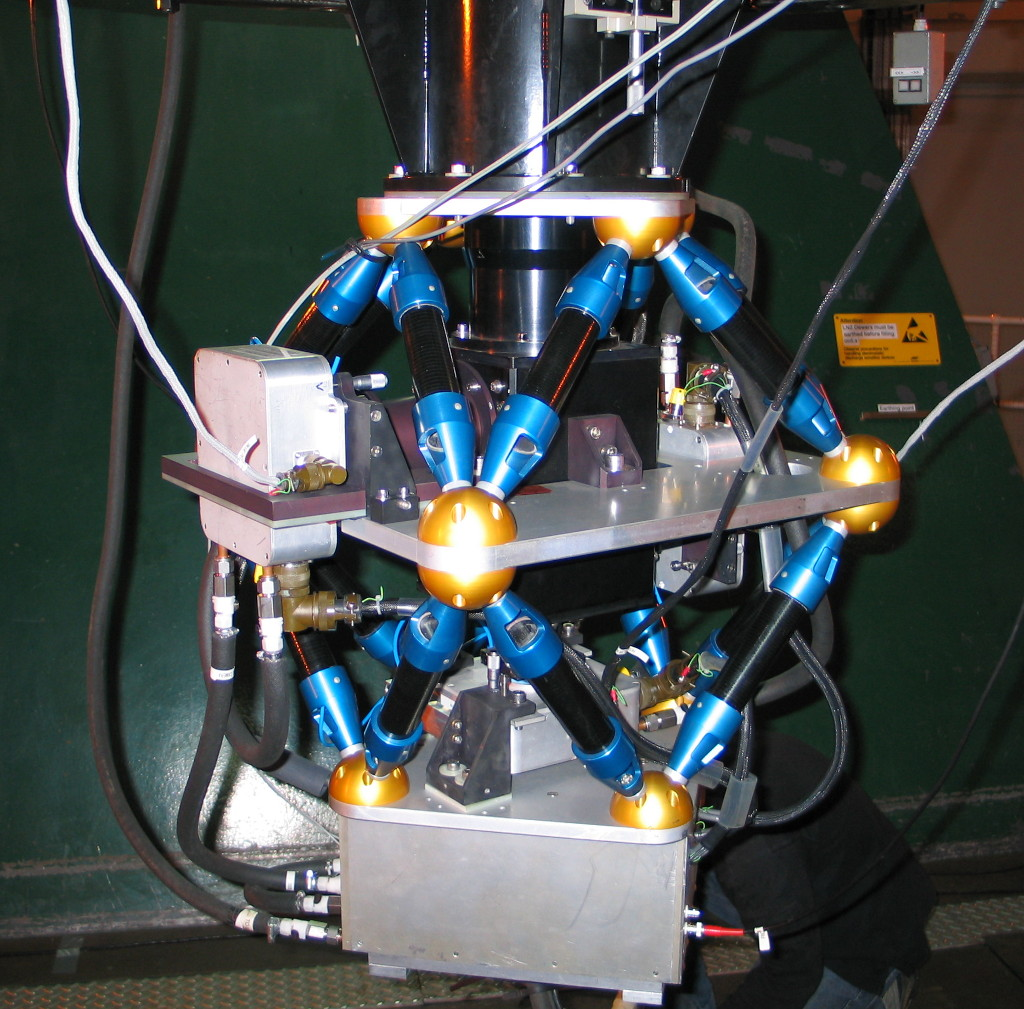
\includegraphics[width=90mm]{images/IMG_0121_scaled.JPG}
\caption{The Ultracam being commissioned in May 2002.}
\label{fig1}
\end{figure}

A key aspect of the design of the camera is its ability to perform at high cadence. It is possible to have the camera read-out at up to 500Hz (frames per channel per second) \cite{dhillon07}. This makes the camera useful for observations of rapid transient events and accurate timing. Although the camera is not often used in this very high speed mode, there are a few observing runs where the camera has been operating with exposure times of approximately 0.005 seconds. These runs are described in chapter~\ref{chap:results}.

The filters for each channel can be modified. In usual configurations the SDSS filter (u, g, r, i, z) set are used, but there are a selection of narrow-band filters that can be substituted. Depending on the science measurements that the observer is trying to perform, these filters will be changed.   

Each CCD has a total pixel area of 2057x1024 pixels. Half of these pixels are masked and never exposed to light. They are used as a temporary buffer for reading out the chip. CCD detectors are read out serially, but in order to decrease the time between exposures, the full image can be moved to the blanked out area of the chip and this can then be read out while the un-masked area of the chip is once again exposed to light. 

\begin{figure}[!h]
\centering
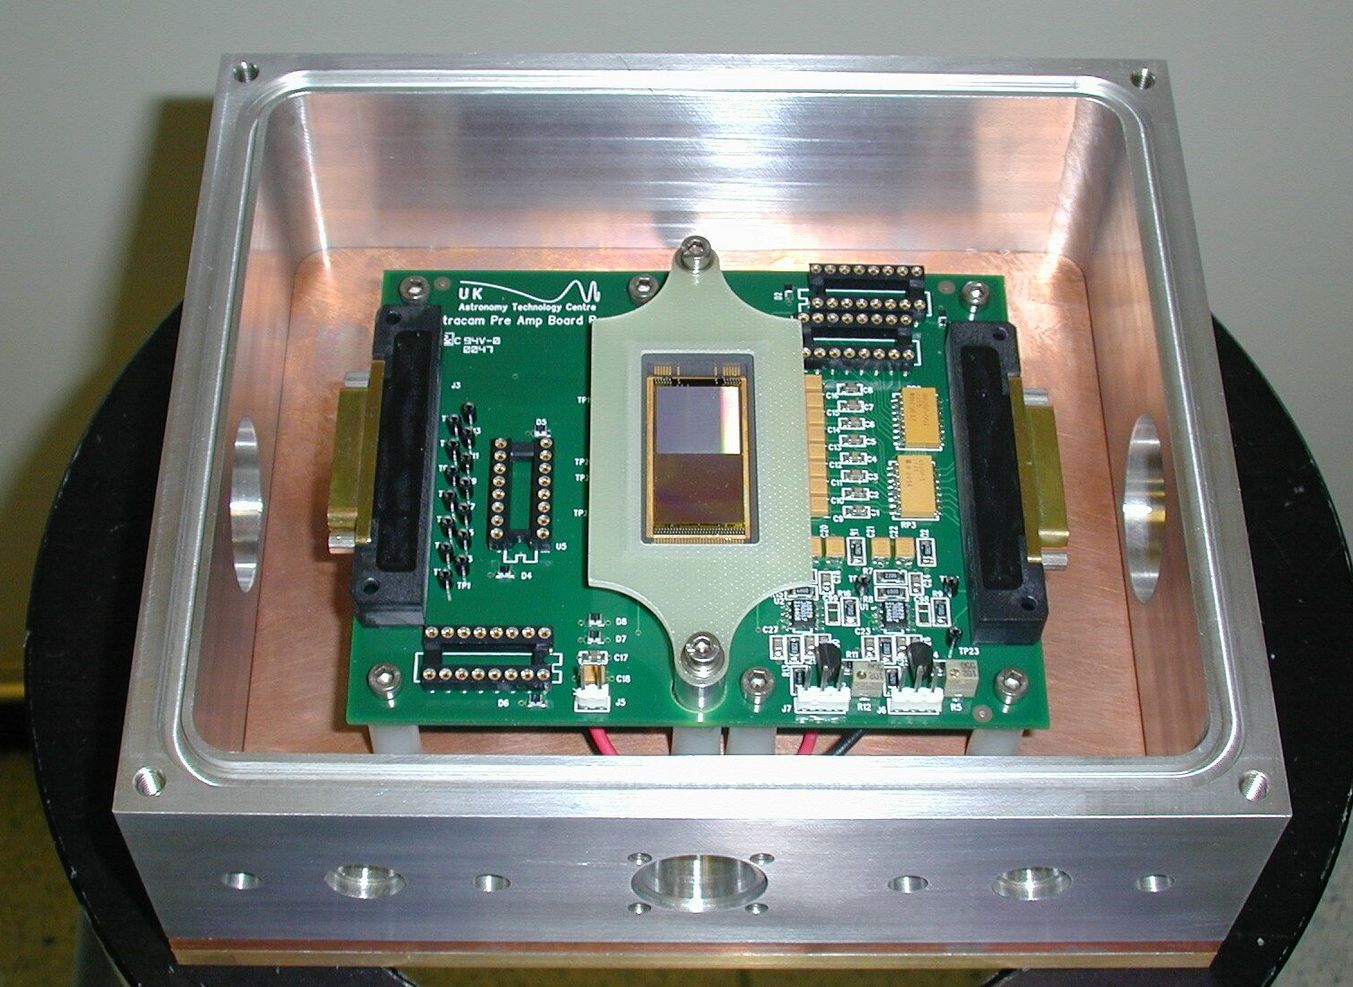
\includegraphics[width=90mm]{images/ccd.png}
\caption{One of the three CCD detectors. The masked-off area is visible in the lower half of the chip surface.}
\label{fig2}
\end{figure}

ULTRACAM gives the observer the ability to reduce the amount of the detector that is used for the exposure. This reduces the readout time of the chip and enables the high cadence. Reducing the number of pixels exposed also decreases the amount of data storage needed for the run. The observer can define pairs of \emph{windows} that are centered on their objects of interest. By making the windows suitably small, the observer can use the camera in extremely high cadence mode. 

\subsection{Drift mode}
The highest cadence mode is called \emph{Drift mode}. This mode uses the masked area of the CCD chip to store several exposures simultaneously. Only the portion of the CCD that is exposed is shifted into the masked area of the CCD meaning that the unmaksed area is ready to be re-exposed more quickly. This mode requires that only the lower portion of the detector, close to the boundary of the masked and un-masked areas, is exposed. Due to the geometry of this readout mode, it is necessary that the exposed area of the CCD is immediately adjacent to boundary with the masked-off section of the chip. This means that the camera will have to be rotated so that the target object (and a suitable comparison star) are positioned correctly. The ULTRACAM is therefore designed to be rotated. For any particular run, it is possible that we can have \emph{any} orientation ($0-180^{\circ}$) of the camera relative to the sky coordinates. This is an important factor to remember when we try to find astrometric solutions for the runs.    

\begin{figure}
  \centering
  \setlength{\fboxsep}{0pt}
  \setlength{\fboxrule}{1pt}
  \fbox{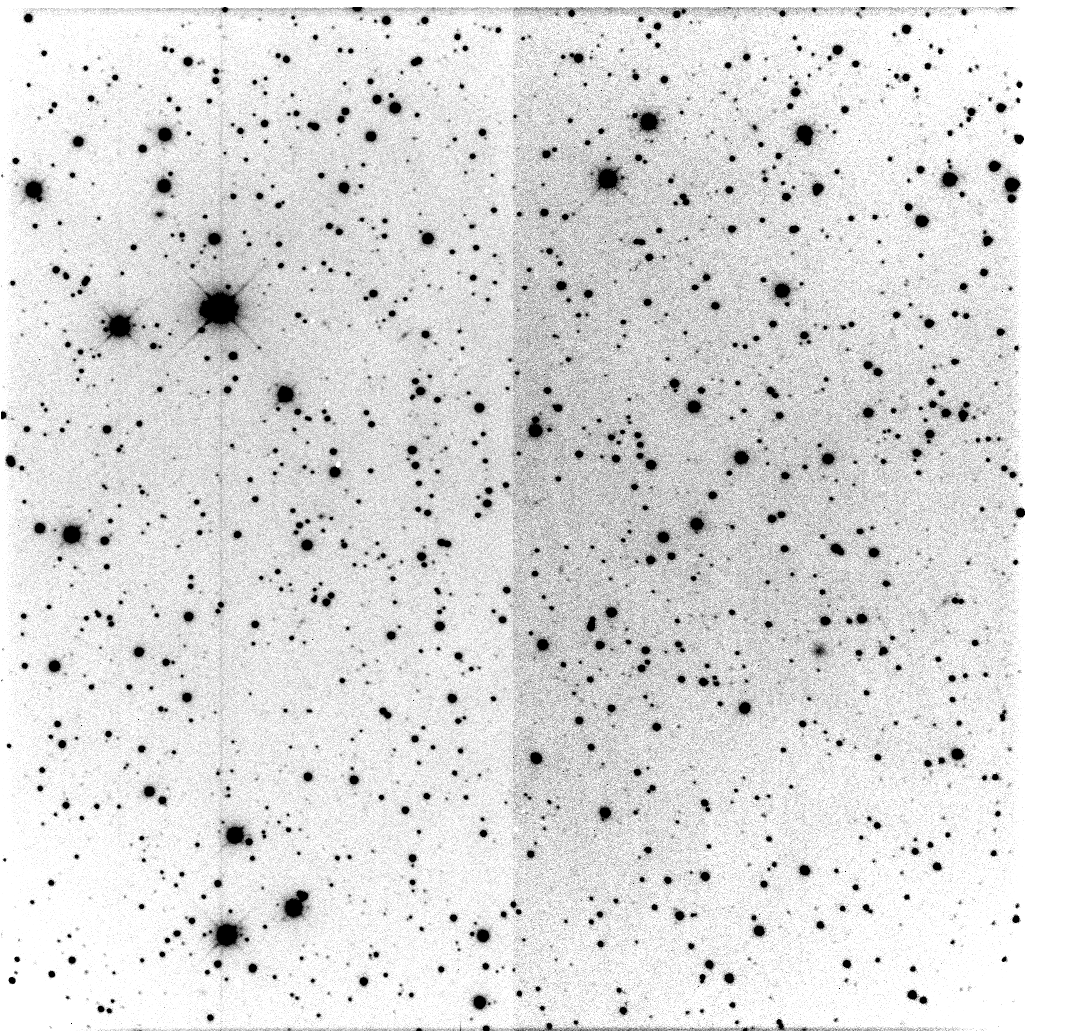
\includegraphics[width=120mm]{images/run010_r_inverted.png}}
  \caption{A 'fully' exposed CCD with 1 pair of windows (512x1024 pixels each)}
  \label{fig:KOI-824}
\end{figure}

\begin{figure}  
  \centering
  \setlength{\fboxsep}{0pt}
  \setlength{\fboxrule}{1pt}
  \fbox{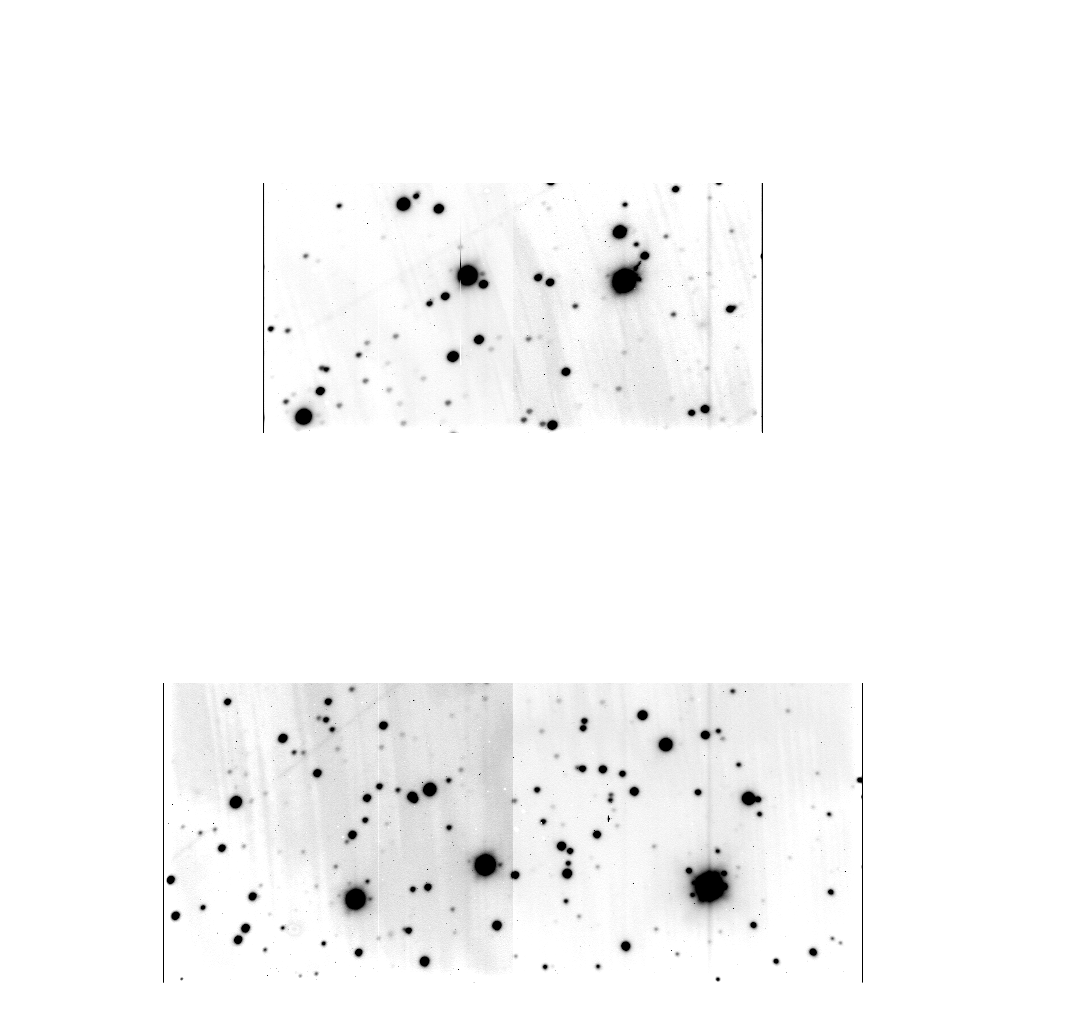
\includegraphics[width=120mm]{images/run016_r_inverted.png}}
  \caption{A 'masked' exposure with 2 pairs of windows (350x300 and 250x250 pixels each, respectively)}
  \label{fig:V713Cep}
\end{figure}

\begin{figure}  
  \centering
  \setlength{\fboxsep}{0pt}
  \setlength{\fboxrule}{1pt}
  \fbox{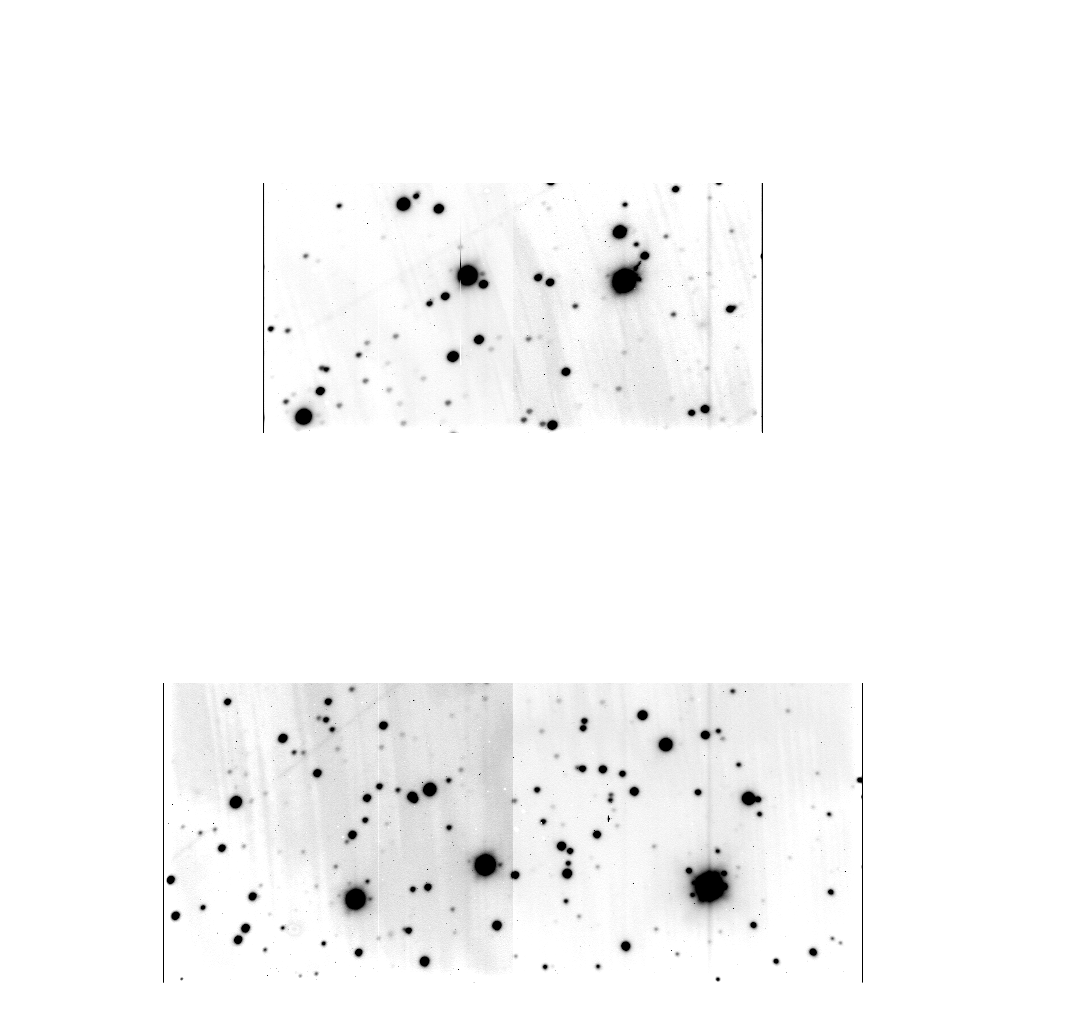
\includegraphics[width=120mm]{images/run016_r_inverted.png}}
  \caption{The camera operating in \emph{drift-mode}. Note the small windows (?x?) located at the bottom of the imaging area. }
  \label{fig:V713Cep}
\end{figure}


More details on the camera design and operation can be found in \cite{dhillon07}.

\subsection{Observation and data recording}

Usually the camera remains installed on the telescope for a week or so and is used for observations on consecutive nights. During the night there are several \emph{runs} made. A \emph{run} can be defined as a period when the camera is active and gathering data. Not all runs are used for gathering \emph{scientific} data. Some runs are used for target acquisition and camera calibration purposes. 

The types of runs are: 
\begin{itemize}
	\item \emph{Science run}: These are the runs that contain the valuable scientific data. They usually comprise the longest portions of the observations during the night, unless the camera is having difficulties or adverse conditions are preventing useful astronomical observations.
	\item \emph{Acquisition run}: These are runs, usually of short duration (ie a few minutes) during which the telescope is being moved in order to place the candidate object(s) in the field of view. The camera may also be rotated in order to align the CCD such that the targets avoid `bad' pixels or are near to the lower boundary of the detector (eg for high speed readout in Drift mode). 
	\item \emph{Sky-flats}: At the start and the end of the night (usually during twilight) the observer will take a few runs to create \emph{sky-flats} that will be used later for calibrating the variations in pixel sensitivity across each of the detectors.  Sky-flats are generated by exposing the camera to patches of sky during the twilight. 
	\item \emph{Bias}: A short run to build calibration readings for measuring the bias of the detector. This bias will be subtracted from the data during the reduction. 
	\item \emph{Timing calibration run}: One way to check the timing measurments of the camera is to take frames of a well-known rapidly oscillating source. For example, the Crab Pulsar (PSR B0531+21). The timing of the pulses as measured by the camera can be compared to the expected times for the pulsar. This is used as a standard clock for timing calibration.
\end{itemize}

\subsection{The data archive}
At the time of writing, the ULTRACAM data archive comprises of about 10 terabytes of saved data. This can be broken down as:
\begin{itemize}
	\item \emph{390} nights on which ULTRACAM was operational at a telescope.
	\item \emph{12 256} runs, including Science, Acquisition runs, etc as listed above. 
	\item \emph{119 817 742} frames in total. This is total includes all the frames for each channel; red, green and blue.
	\item \emph{10 181 269 485 298} bytes of raw image data.
\end{itemize} 
The data set is relatively large and is housed on a network mounted storage device that is only available through the internal university computer network. This means that it is not possible to access this data from remote locations (for example, by research collaborators in different institutions). If a researcher needs to see some data, then they need to contact a member of department at Warwick or Sheffield and request a data reduction. There is no means to explore the ULTRACAM data set from their remote location. It is clear that providing a simple means of accessing the data from remote locations would benefit all of the research collaborators. 

\subsection{Data reduction}
Tom Marsh at the University of Warwick has developed a set of software tools that allow the observer to reduce the data in `real-time'. This allows observers to review the data while it is being gathered at the telescope. This serves as a `preview' for the observer and allows adjustments to be made during the run. After the run, the raw data is copied to the archive and this can be used for reductions later. This can happen the following day, or much later when the observer has returned from the telescope site. This data archive can be `re-reduced' at any time as all of the raw data is stored in the archive. 

The current data reduction process for ULTRACAM is designed to produce three colour light curves from the raw image data. The pipeline consists of the following stages:
\begin{enumerate}
	\item Producing \emph{bias} frames that are used the calibrate the CCD detector's thermal noise characteristics. 
	\item Producing \emph{flat-fields} to calibrate the pixel sensitivity of each of the 3 CCD detectors. These flat-fields are subtracted from the image data during the reduction process.
	\item Defining \emph{apertures} for the objects of interest in the run. This step requires manually chosing the objects of interest in the frames and defining the aperture sizes for each object. Apertures are independently set for each channel (r, g, b). 
	\item Running the \emph{reduction} software. This code uses the apertures defined in the previous step and measures the flux of each object in each colour. The software is able to track changes in the object's size and shape due to changes in the point spread function (PSF) by scaling the virtual aperture. It is also able to track small deviations in the positions of the objects. 
\end{enumerate} 
Although this process is not particularly cumbersome, it \emph{does} include some manual steps and it does not scale well when there are a large number of runs to be processed or if there are many target objects on each frame. The example in Fig. \ref{fig:KOI-824} contains more than 1000 objects. Manually defining apertures for each of these objects in each channel is not really practical. An automated method would enable data reduction for all of the objects captured in each run without manual intervention. 

\subsection{Motivation for an automated pipeline}
ULTRACAM has recorded a large amount of photometric data at some of the world's best sites and largest telescopes. Since the CCD captures more objects than the observer is strictly interested in, there is a good chance that some objects of astronomical interest have been captured by ULTRACAM, but not been noticed during the reduction process. By automating the reduction pipeline we can produce reduced photometry for \emph{all} of the objects captured by ULTRACAM and search through the archive to find new objects of interest. 

An automated pipeline can be run on the data immediately after the run is complete, allowing observers at the telescope to review their results during the course of their observing run. It will also allow collaborators who are not physically at the observatory to browse the data as it is coming in. This enables a strong collaboration with onsite and offsite teams during a run. 

er
\section{Automating the Ultracam pipeline}

\subsection{Project goals}
The outcome of this MSc project will be a software pipeline that provides an automated way of reducing the raw data from ULTRACAM.  The key outputs will be field identification through astrometry, deep image generation and light-curve reduction for all of the science runs in the data. 

The final product should allow researchers to quickly browse the reduced data and examine light-curves of each object in all of the 
runs. The light-curves and runs should also be graded in terms of quality (eg seeing, atmospheric transmission, etc) 

The \emph{minimum} goals for this project are:
\begin{itemize}
	\item An \emph{automated pipeline} which can process ULTRACAM data to obtain light-curves for all objects within the field of any science run. This data will include light-curves for all objects and all channels in each run. An indicator of quality of the run will also be provided. 
	\item A \emph{light-curve} browser allowing a researcher to query and browse the Ultracam archive by date, object and position.
	\item \emph{Deep images} of the observed field for all three channels for each run, based on stacking of frames in the run. The quality of the image will be ensured by discarding poor frames and taking into account movement of the frames due to tracking- and/or atmospheric effects. 
\end{itemize}

In addition to these minimum requirements, it would be \emph{desirable} to have results for:

\begin{itemize}
	\item \emph{Full photometric reduction}. If the quality of the automated reduction is not high enough for science research, then the pipeline could include a stage that prepares and runs the current Ultracam pipeline reduction process for more accurate reductions.
	\item \emph{Identification} of moving objects seen in the run. For example, these might be Kuiper belt objects (moving at a few arcseconds per hour).
	\item \emph{Automated alerts} triggered when a interesting (variable or transient) light curve is detected by the pipeline. 
	\item \emph{Movies} (in .mp4 format) of the run displayed in the light-curve browser. 
\end{itemize}

\subsection{Approach}
The key step in automating the Ultracam pipeline is finding a reliable way of identifying all of the objects in a run and tracking them across all of the frames. It is also necessary to identify the same objects in each of the three colour channels. 

\subsubsection{Source extraction}
A popular software tool used for source extraction is SExtractor \cite{bertin}. SExtractor is able to process an image field and produce a catalog of sources in that field along with a measurement of the flux count of each object. The flux count is calculated after making efforts to account for the background in the field and then fitting a profile to the object. \emph{Comment: Will need a full chapter on this in the thesis, including tweaks to the configuration parameters of SExtractor and how it affects the results.}

\subsubsection{Algorithm}
The stages of the reduction process are as follows:
\begin{enumerate}
	\item Stage 1: Create a list of objects found in the run. 
	\begin{enumerate}
		\item Read the raw image file, containing all frames for a particular run.
		\item Initialise an empty list of objects
		\item For each frame in the run
		\begin{enumerate}
			\item For each colour channel in the frame
			\item Extract each window from the frame
			\item Send the image to the SExtractor software
			\item Read the results of the source extraction process, including pixel position and flux measurements for each object
			\item For each object returned
			\begin{enumerate} 
				\item Try to match this object with one already in the list, based on nearest distance.
				\item If the object is not already in a list, add this object to the list as a \emph{new} object.
			\end{enumerate}
		\end{enumerate}
		\item Store the list of objects for each of the three channels.
	\end{enumerate}
	\item Stage 2: Filter this list, removing objects that are likely to be artifacts. This is done by looking for objects that do not persist across more than a pre-defined percentage of frames; and objects that have a size approximately equal to one pixel. 
	\item Stage 3: Produce catalogs of the objects ordered by 'brightness' as measured by the flux estimate from SExtractor. Pass these catalogs to the Astrometry.net library to resolve the WCS solution for the fields. Since the three channels have a very slightly different view and different distortions of the image, their WCS solutions will differ by a small amount.
	\item Stage 4: Using the WCS solutions, merge the three catalogs to 'cross-identify' each object across the three channels. This may seem to be a trivial step for many ULTRACAM runs because the differences in the fields from channel to channel are minor, however in crowded fields such as the one shown in Fig. \ref{fig:KOI-824} simply matching objects based on their pixel coordinates is not enough to disambiguate them.
	\item Stage 5: Produce deep images for each channel and export to a web-viewable format, such as PNG. 
	\item Stage 6: Create .json data files and HTML files to enable viewing the output of the run through a web browser. 
	\item Stage 7: Publish this 'web-enabled' data to a web site that is accessible outside of the university network.  
		
\end{enumerate}

\begin{figure}[!h]
	\centering
	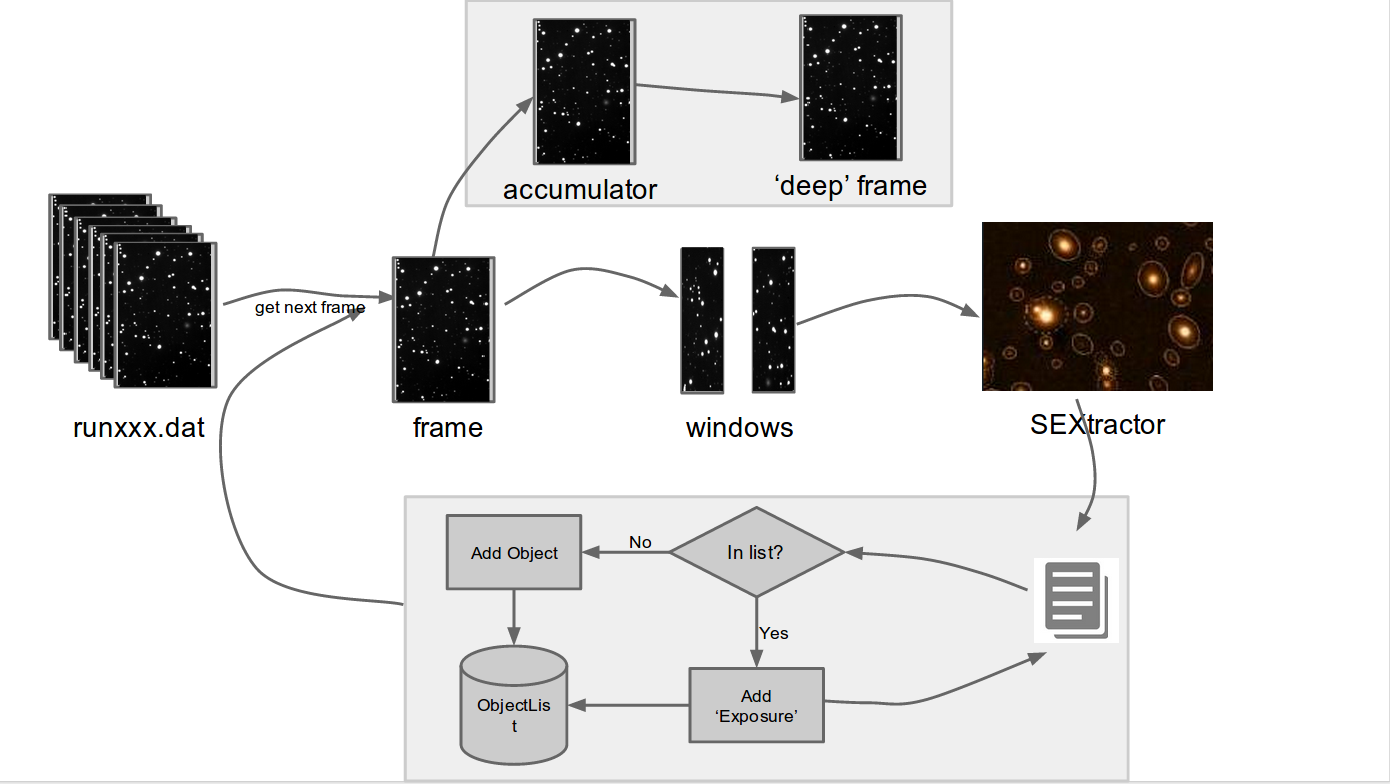
\includegraphics[width=130mm]{images/flowchart.png}
	\caption{Schematic of Stage 1 of the pipeline.}
	\label{flowchart}
\end{figure}


\begin{figure}[!h]
	\centering
	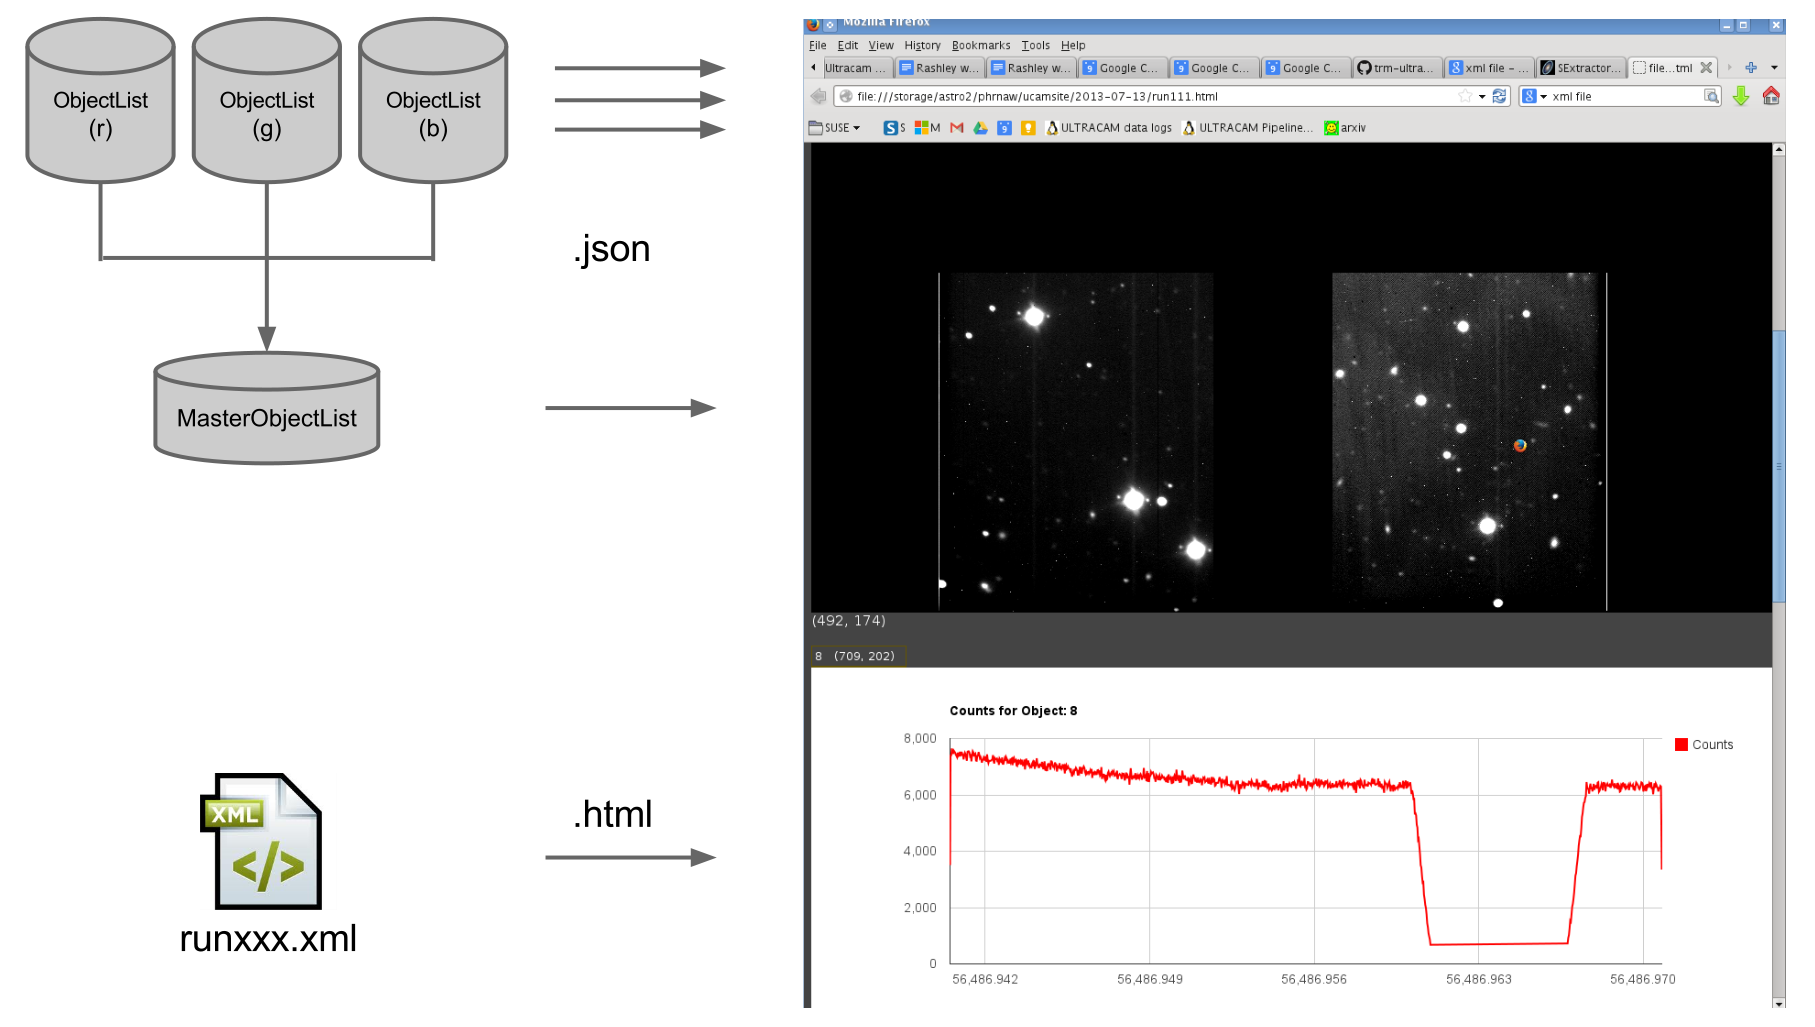
\includegraphics[width=130mm]{images/webpublish.png}
	\caption{Schematic of Stage 6 and 7 of the pipeline.}
	\label{webpublish}
\end{figure}



\subsection{User Interface}
The core `visible product' of the project will be a website that allows a user to browse all of the data in the ULTRACAM archive. The key features of this website will be:

\begin{itemize}
	\item A \emph{search} interface to allow the user to query the archive by object identifier and/or world coordinates (right ascension, declination). 
	\item A catalog of runs organised by calendar date, containing \emph{thumbnail images} of the fields.
	\item For each run, a web page that shows the user:
	\begin{itemize}
		\item the \emph{deep images} of the field in individual colours and also a combined (r,g,b) image.
		\item the \emph{light-curves} of each object as the user clicks on the object with the mouse. 
		\item \emph{previews} of the light curves as the user 'hovers-over' the object with the mouse. 
	\end{itemize}
	\item light-curves should be plotted as absolute measured flux or a \emph{relative flux} compared to some other objects in the field. 
	\item the web page should also allow the user to \emph{export} the data to a standard format, such as FITs.
	
\end{itemize}
See Fig. \ref{browser} for an example of the web-page. 


\begin{figure}[!h]
	\centering
	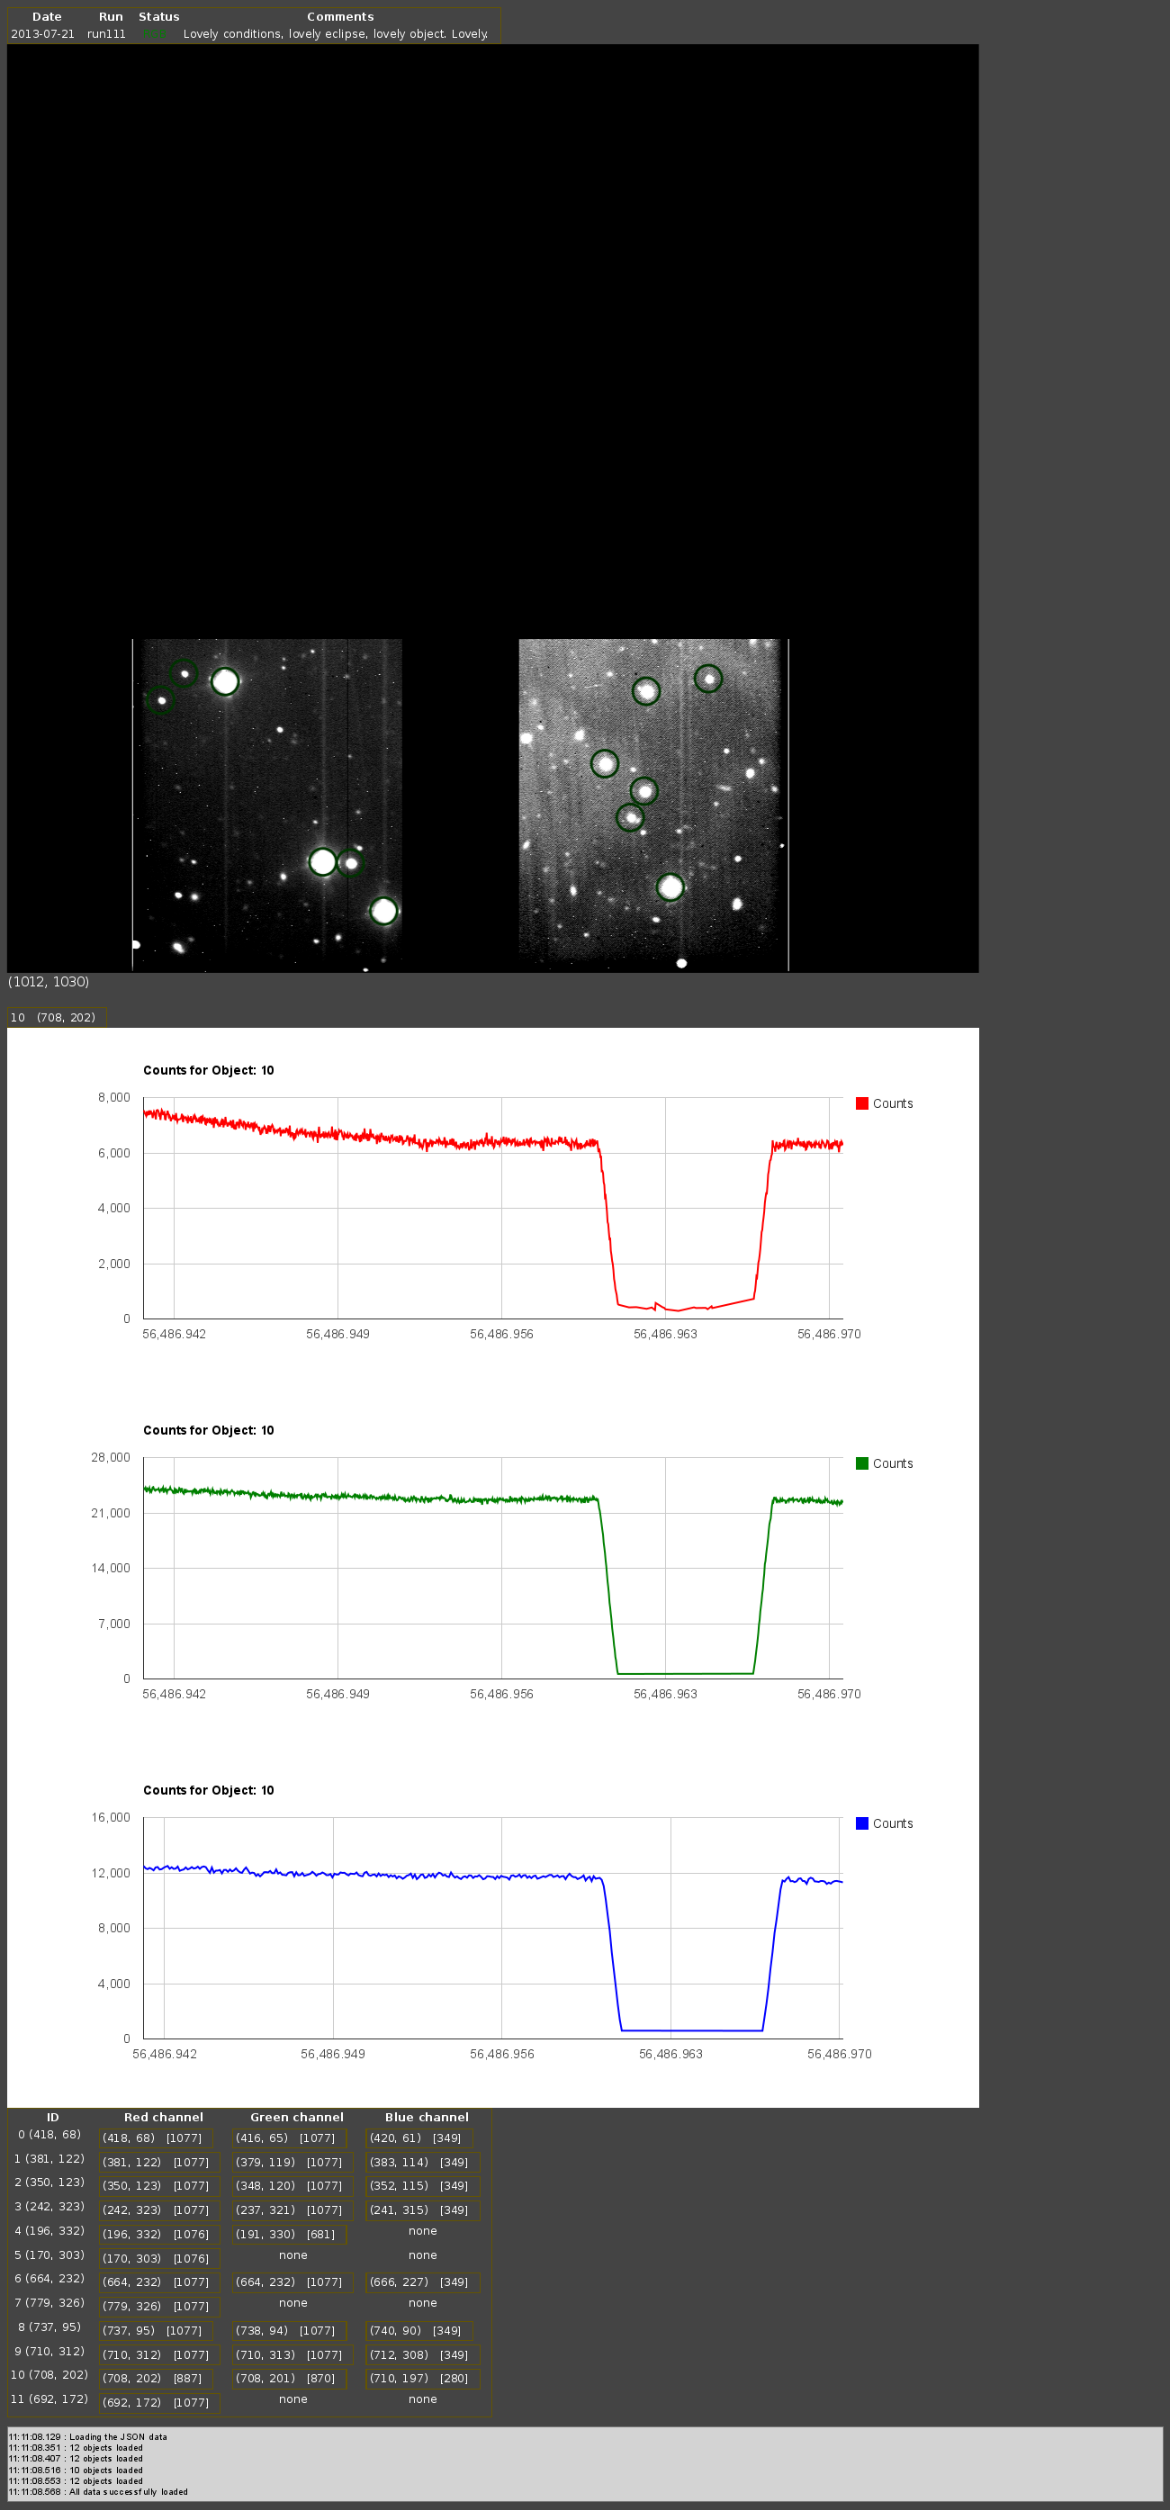
\includegraphics[width=90mm]{images/browser.png}
	\caption{Preview of the webpage.}
	\label{browser}
\end{figure}

\section{Progress so far}
At the moment, the software for the pipeline as at a stage where it is able to produce light curves for many of the runs in the data archive. This means that, given a run, it is possible to produce a web-page (as described above) that has deep images for the field and light curves for all of the objects in the field. Therefore, at its most basic, the pipeline `works', however there is still significant work to be done. 

\subsection{WCS solution}
After some ad-hoc tests using \emph{SCAMP \cite{scamp}} and \emph{Astrometry.net \cite{astrometry}} it seemed that the Astrometry.net software was more reliable at finding good WCS solutions to the fields. The software was downloaded to a local machine (including the extensive index files) and compiled. At the moment, this is now part of the pipeline but it does not consistently find WCS solutions for all of the fields. 

There are several difficulties in reliably finding a WCS solution for the fields.  These are:
\begin{itemize}
	\item \emph{Lack of pointing data}: The Ultracam system does not integrate with the pointing software of any of the telescopes and does not get pointing information automatically. We rely on the observer to enter a name of the candidate object for each run and then, when the data is archived, a \emph{SIMBAD} lookup is used. This gives us a world coordinate that is somewhere in the field, but it is not known which object (or pixel location) this applies to.  
	\item \emph{Field rotation}: Since the Ultracam can be rotated about the optical axis to allow for optimal alignment of the objects, this means that the field of view can be at any arbitrary rotation giving an extra degree of freedom to the matching task. 
	\item \emph{Windows}: Many ULTRACAM runs are configured to use only portions of the CCD area. You can see an example of this in Fig.  \ref{fig:V713Cep}. This means that there is an incomplete view of the sky for that field. When trying to match to existing indexes, there could be important, bright objects that are in the index file, but do not appear in the Ultracam field due to the masking caused by the windows.
	\item \emph{Sparse fields}: On uncrowded fields, we might only have 4-5 objects that can be used for field identification. 
	\item \emph{Very small windows}: Some runs, particularly ones in high cadence mode, use very small windows (eg 172x156 pixels) in order to decrease readout time. This means that the Ultracam images might only contain two objects or so. This makes matching to a reference catalog impossible. 
	\item \emph{Choice of reference index by colour}: The Astrometry.net software uses 2MASS and Tycho-2 reference catalogs by default. These are based on infra-red and V magnitudes. This means that the blue channel (which is often using the SDSS u filter) might not match the reference indexes. Indeed, current tests often end with a match in red, a match in green and no match in blue. 
\end{itemize}

The current line of investigation in the project is to try to use positive matches in the red and/or green channel to 'seed' the search for matches in the blue channel. If this doesn't work, it may be worthwhile to seek alternative (bluer) reference catalogs. 

For sparse fields, it might be worth looking for deeper reference catalogs. 

For the very sparse fields, with 2 to 3 objects on them, it is unlikely that a WCS solution can be found. This is probably not a problem as the number of objects is so low, there is unlikely to be any ambiguity in cross-matching the object across the channels and combining the light-curves can be performed simply by matching based on the object's pixel coordinates alone.  


\subsection{Quality of the photometry}
The photometry of the objects is simply the flux estimate produced by the SExtractor software and has not been evaluated in terms of its accuracy relative to the existing Ultracam reduction pipeline. Also, there has been no effort to look at the errors in flux measurements (as estimated by SExtractor). This work still needs to be done. 

A preliminary check of photometry is shown in Fig. \ref{fig:V834Cen}. 

\begin{figure}[!h]
	\centering
	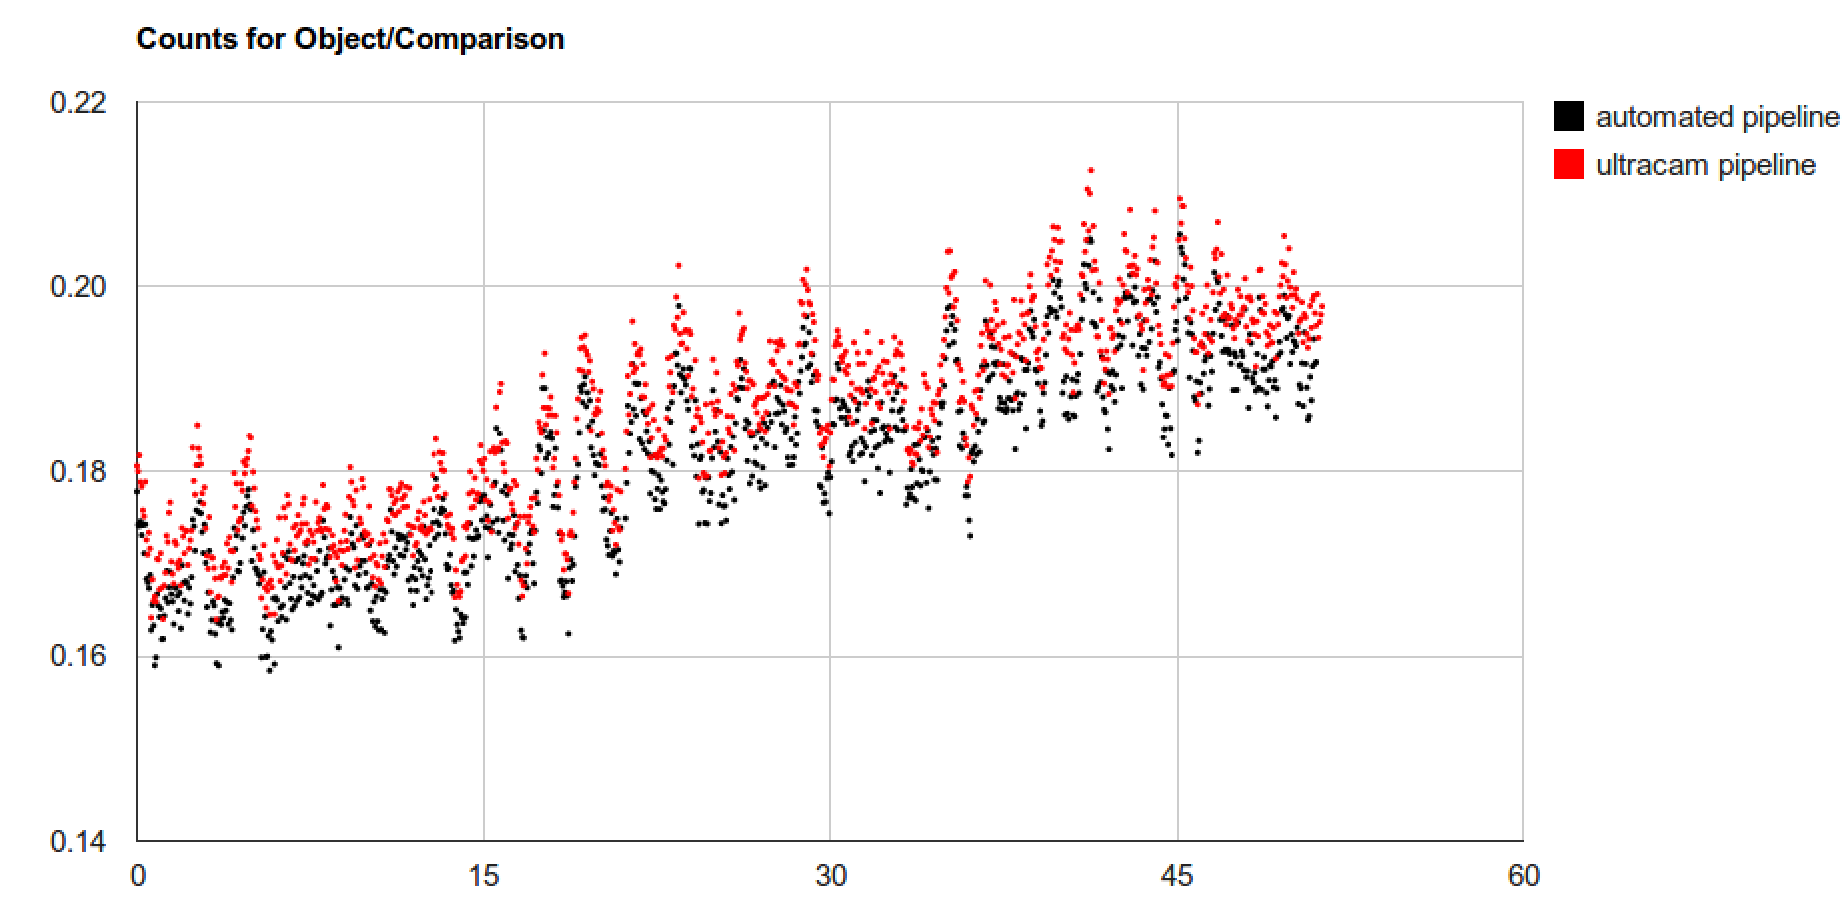
\includegraphics[width=120mm]{images/V834Cen.png}
	\caption{Comparison of the photometry of the Ultracam pipeline with the new automated pipeline (this project). The data shows the 'r' band photometry for 60 seconds in the light-curve of the polar V834 Cen.}
	\label{fig:V834Cen}
\end{figure}

\subsection{Run classification}
Due to the diversity of data in the Ultracam archive, not all of the runs can be processed in the same way. Crowded fields with full-frame exposure need to be treated in a different way to high cadence runs of only a few objects. SExtractor parameters need to be tweaked in order to get the best results depending on the nature of the run. At the moment, this step is done manually and with some `trial and error'. If the pipeline is to run in a truly automated way, then it needs to be able to adapt to this diverse data and perform a `run classification'. This classification step should also attempt to identify non-science runs, such as flat-fields, biases and acquisition runs and deal with them appropriately. Some acquisition runs often become real science runs and contain valuable data. 

\subsection{Search interface}
At the moment, since there is no robust solution for solving WCS coordinates (yet), the search interface has not been built. It should be possible to query the archive using world coordinates. A WCS solution should be available for every science (and potentially also acquistion) run in order to build the search index (within the limitations mentioned above). 

\subsection{Cover the entire data archive} 
The browseable archive (the product of this project) should cover the entire ULTRACAM archive, from May 2002 to the present. Once some of the remaining issues have been resolved (mainly WCS solutions and Run classifications) then the pipeline should be set to run across the entire data set. 

